\documentclass[aps,prl,reprint,groupedaddress,onecolumn,superscriptaddress]{revtex4-2}
\usepackage{graphicx}% Include figure files
\usepackage{dcolumn}% Align table columns on decimal point
\usepackage{bm}% bold math
\usepackage{amsmath}
\usepackage{siunitx}
\usepackage{enumitem}
\usepackage{booktabs} % For better tables

\begin{document}

\title{Bullet-Point List of the Barium Network Paper}
\date{\today}

\maketitle

\section{Principle of Operation: \\ Dual-Wavelength Interferometric Refractometer}

\subsection{Innovation Rationale}
\begin{itemize}
    \item \textbf{Core Concept}: Quantum-network-compatible atmospheric monitoring requires unprecedented refractive index precision ($\delta n \sim 10^{-9}$) at quantum-critical wavelengths
    \item \textbf{Technical Innovation}: Modified NIST LM10 design optimized for:
    \begin{itemize}
        \item Dual-wavelength operation
        \item Metropolitan-scale optical path difference
        \item Environmental robustness for field deployment
    \end{itemize}
    \item \textbf{Quantum Integration}: Direct linkage to trapped-ion frequency standards enables SI-traceable metrology
    \item \textbf{Application Focus}: Enables precise phase compensation for quantum key distribution and quantum memory operations
\end{itemize}

\subsection{Operating Principle}
\begin{itemize}
    \item Simultaneous fringe counting at both wavelengths provides differential measurement
    \item Environmental perturbations affect both beams equally, common-mode rejection enhances sensitivity
    \item Ratio-metric approach cancels mechanical vibrations and common-path fluctuations
    \item Quantum-referenced lasers provide absolute frequency calibration with $<$\SI{1}{\kilo\hertz} stability
    \item Real-time environmental monitoring enables predictive phase noise compensation
\end{itemize}

\section{Experimental Setup}

\subsection{Interferometer System}
\begin{itemize}
    \item \textbf{Core Design}: Dual-wavelength Michelson interferometer
    \item \textbf{Optical Path Difference}: \SI{4.2}{\meter} (representative of metropolitan-scale quantum links)
    \item \textbf{Vibration Isolation}: Air-floated mirror stage (\SI{120}{\centi\meter} travel) minimizes vibrational noise
    \item \textbf{Detection System}: 
    \begin{itemize}
        \item Si photodiode for \SI{780}{\nano\meter} reference beam
        \item InGaAs photodiode for \SI{1762}{\nano\meter} probe beam
    \end{itemize}
    \item \textbf{Electronics}: Hewlett Packard 53131A frequency counter, two channels, 10 digits/s resolution, \SI{225}{\mega\hertz} bandwidth
\end{itemize}

\subsection{Quantum References}

\subsubsection{Rb Laser (\SI{780}{\nano\meter} Reference)}
\begin{itemize}
    \item Stabilized via saturation absorption spectroscopy on the $5S_{1/2} \rightarrow 5P_{3/2}$ transition of $^{87}\text{Rb}$
    \item \textbf{Uncertainty \& Stability Analysis:}
    \begin{itemize}
        \item Frequency stability: \SI{\sim100}{\kilo\hertz} linewidth (homodyne measurement)
        \item Short-term (10 s): contributes $\delta n \sim 10^{-10}$ to refractive index uncertainty
        \item Medium-term (10 hours): potential slow drift contributes $\delta n \sim 10^{-9}$ (measured with Highfinesse wavemeter)
        \item Long-term (10 days): negligible with periodic recalibration
    \end{itemize}
\end{itemize}

\subsubsection{Ba$^+$ Laser (\SI{1762}{\nano\meter} Probe)}
\begin{itemize}
    \item Primary reference: single trapped $^{138}\text{Ba}^+$ ion, stabilized to the $6S_{1/2} \rightarrow 5D_{5/2}$ electric quadrupole transition
    \item Short-term stability provided by a ULE cavity; systematic uncertainties $<$ \num{1e-13}
    \item \textbf{Uncertainty \& Stability Analysis:}
    \begin{itemize}
        \item Frequency stability: $<$ \SI{1}{\kilo\hertz} (from $^{138}\text{Ba}^+$ ion electric quadrupole transition resolution)
        \item All time scales: contributes $\delta n < 10^{-12}$ to refractive index uncertainty
        \item Negligible impact compared to system residual error of \num{1.2e-9}
    \end{itemize}
\end{itemize}

\subsection{Supporting Systems}

\subsubsection{Ambient Monitoring}
\begin{itemize}
    \item BME280 sensor, co-located with interferometer beam path (within \SI{10}{\centi\meter})
    \item Temperature: uncertainty \SI{\pm 1}{\degreeCelsius}
    \item Humidity: uncertainty \SI{\pm 3}{\percent} RH
    \item Pressure: uncertainty \SI{\pm 0.6}{\hecto\pascal}
    \item Backup sensors: DHT22 (\SI{\pm 0.5}{\degreeCelsius}, \SI{\pm 1}{\percent} RH)
    \item \textbf{Uncertainty \& Stability Analysis:}
    \begin{itemize}
        \item Temperature uncertainty: $\delta n_T \approx 8.94\times10^{-7}$ (dominant error source)
        \item Humidity uncertainty: $\delta n_H \approx 5.3\times10^{-8}$
        \item Pressure uncertainty: $\delta n_P \approx 1.5\times10^{-7}$
        \item Total systematic uncertainty: \num{2.12e-7} (consistent with documented value)
        \item Time scale impact: affects all time scales equally, requires model correction
    \end{itemize}
\end{itemize}

\subsubsection{Timing Synchronization}
\begin{itemize}
    \item GPS-disciplined oscillator (\SI{10}{\mega\hertz} universal timebase) synchronizes all data acquisition
    \item Central time-series database (InfluxDB) for correlated analysis
    \item \textbf{Uncertainty \& Stability Analysis:}
    \begin{itemize}
        \item Allan deviation: \SI{2.03e-11} (10 s), \SI{3.09e-12} (100 s), \SI{8.69e-13} (1000 s), \SI{7.81e-13} (10000 s)
        \item Short-term (10 s): contributes $\delta n \sim 10^{-11}$ (negligible)
        \item Medium/Long-term: contributes $\delta n \sim 10^{-13}$ (negligible)
        \item Excellent long-term stability enables precise time-series correlation
    \end{itemize}
\end{itemize}

\section{Data Collection and Processing}

\subsection{Dataset Composition}
\begin{itemize}
    \item Training Dataset: \num{89106} synchronized measurements
    \item Validation Dataset: \num{46999} synchronized measurements (\SI{15}{days}, temporally separated)
\end{itemize}

\subsection{Environmental Conditions}
\begin{itemize}
    \item Temperature range: \SIrange{15}{35}{\degreeCelsius}
    \item Relative humidity: \SIrange{20}{45}{\percent}
    \item Pressure range: \SIrange{965}{1000}{\hecto\pascal}
\end{itemize}

\subsection{Sampling Strategy}
\begin{itemize}
    \item Environmental parameters: \SI{1}{\hertz} sampling rate
    \item Interferometric fringes: \SI{\sim 0.06}{\hertz} (every \SI{17}{\second}, limited by integration time)
\end{itemize}

\subsection{Data Preprocessing}
\begin{itemize}
    \item Timestamp alignment via linear interpolation
    \item Outlier removal using adaptive statistical thresholds
    \item Quality control based on GPS timing consistency
\end{itemize}

\section{Results and Analysis}

\subsection{Refractive Index Modeling}

\subsubsection{Calculation Method}
\begin{itemize}
    \item $$n_{1762} = \frac{n_{780}}{\text{Ratio}} \frac{f_{780}}{f_{1762}}$$, where Ratio = $N_{780}/N_{1762}$ (fringe counts ratio)
    \item $n_{780}$ computed from environmental parameters using Ciddor equation
\end{itemize}

\subsubsection{Regression Analysis}
\begin{itemize}
    \item Multivariate linear regression: $n = \alpha_0 + \alpha_T T + \alpha_H H + \alpha_P P$
    \item Goodness-of-fit: $R^2 = \num{0.996}$, F-statistic = \num{7.530e6} ($p < \num{0.001}$)
    \item Residual standard error: $\sigma_n \approx \num{1.2e-9}$
\end{itemize}

\subsubsection{Statistical Validation}
\begin{itemize}
    \item HAC (Heteroskedasticity and Autocorrelation Consistent) standard errors applied (lag = \numrange{18}{37})
    \item Block bootstrap validation (\num{2000} samples, block length = \num{58}) confirmed robustness
    \item Residual diagnostics: Durbin-Watson = \num{1.130}, Breusch-Godfrey LM = \num{29734.5} ($p < \num{0.001}$)
\end{itemize}

\subsection{Refractive Index Coefficients at \SI{1762}{\nano\meter}}

\subsubsection{Experimental Coefficients (with \SI{95}{\percent} HAC CI)}
\begin{itemize}
    \item Temperature ($\alpha_T$): \SI{-8.940e-7}{\per\degreeCelsius} [\num{-8.942e-7}, \num{-8.938e-7}]
    \item Humidity ($\alpha_H$): \SI{-1.780e-8}{\per\percent} [\num{-1.796e-8}, \num{-1.764e-8}]
    \item Pressure ($\alpha_P$): \SI{+2.569e-7}{\per\hecto\pascal} [\num{2.557e-7}, \num{2.581e-7}]
\end{itemize}

\subsubsection{Uncertainty Analysis}
\begin{itemize}
    \item Systematic uncertainty (dominant): \num{2.12e-7} (from spatial/temporal sensor mismatches)
    \item Coefficient precision: $\delta\alpha_T = \num{1.77e-10}$, $\delta\alpha_H = \num{1.81e-10}$, $\delta\alpha_P = \num{1.10e-10}$
\end{itemize}

\subsection{Humidity Sensitivity Enhancement}

\subsubsection{Experimental vs. Theoretical Models}
\begin{itemize}
    \item Measured $\partial n/\partial H = \SI{-1.780e-8}{\per\percent}$
    \item Ciddor: \SI{-1.537e-8}{\per\percent} (\SI{+15.8}{\percent} discrepancy)
    \item Edlén: \SI{-1.526e-8}{\per\percent} (\SI{+16.6}{\percent} discrepancy)
    \item Mathar: \SI{-1.653e-8}{\per\percent} (\SI{+7.7}{\percent} discrepancy)
\end{itemize}

\subsubsection{Physical Mechanism}
\begin{itemize}
    \item Proximity to H$_2$O absorption lines at \SI{1761.0405}{\nano\meter} and \SI{1762.4852}{\nano\meter}
    \item Kramers-Kronig dispersion calculation: predicts \SI{+15.3}{\percent} enhancement over Ciddor
    \item Theoretical $\alpha_H^{\text{theory}} = \SI{-1.772e-8}{\per\percent}$ (within \SI{0.5}{\percent} of experiment)
\end{itemize}

\subsection{Phase Noise Compensation Performance}

\subsubsection{Long-term Performance (\SI{15}{days})}
\begin{itemize}
    \item Phase noise reduction: \SI{80.97}{\percent}
    \item Phase standard deviation: \SI{17.938}{\radian} → \SI{3.414}{\radian} (\num{5.3}× improvement)
    \item Autocorrelation time: \SI{5668}{\second} → \SI{302}{\second}
    \item QEC threshold compliance: \SI{1.2}{\percent} → \SI{9.7}{\percent} of operational time
\end{itemize}

\subsubsection{Short-term Performance (\SI{12}{\hour})}
\begin{itemize}
    \item Phase noise reduction: \SI{60.20}{\percent}
    \item Phase standard deviation: \SI{6.548}{\radian} → \SI{2.606}{\radian} (\num{2.5}× improvement)
    \item Autocorrelation time: \SI{560}{\second} → \SI{1}{\second} (\num{560}× reduction, effective whitening)
    \item QEC threshold compliance: \SI{3.3}{\percent} → \SI{13.3}{\percent} of operational time
\end{itemize}

\subsubsection{Compensation Methodology}
\begin{itemize}
    \item Offline feed-forward subtraction using experimentally determined coefficients
    \item Real-time implementation feasible for quantum network applications
\end{itemize}

\section{Uncertainty and Stability Budget}

\subsection{Multi-Timescale Impact on Refractive Index Measurement}

\begin{table}[ht]
\centering
\caption{Uncertainty contributions at different time scales}
\begin{tabular}{lccc}
\toprule
\textbf{Component} & \textbf{Short-term (10 s)} & \textbf{Medium-term (10 hours)} & \textbf{Long-term (10 days)} \\
\midrule
Rb Laser & \num{e-10} & \num{e-9} & Negligible \\
Ba$^+$ Laser & $<$\num{e-12} & $<$\num{e-12} & $<$\num{e-12} \\
BME280 Sensor & \num{2.12e-7} & \num{2.12e-7} & \num{2.12e-7} \\
GPS Timing & \num{e-11} & \num{e-13} & \num{e-13} \\
\midrule
\textbf{Dominant Source} & \textbf{BME280} & \textbf{BME280 + Rb drift} & \textbf{BME280} \\
\bottomrule
\end{tabular}
\end{table}

\subsection{Key Findings and Recommendations}
\begin{itemize}
    \item The BME280 environmental sensor uncertainty (\num{2.12e-7}) dominates the refractive index error budget across all time scales
    \item $^{138}\text{Ba}^+$ laser stability ($<$\SI{1}{\kilo\hertz}) enables the demonstrated \num{1.2e-9} residual precision
    \item GPS timing stability provides excellent long-term synchronization with negligible impact
    \item \textbf{Improvement Pathway}: Focus on higher-precision environmental sensors to reduce the dominant error source to $10^{-8}$ level
    \item \textbf{Quantum Network Readiness}: System demonstrates sufficient stability for metropolitan-scale quantum communication applications
\end{itemize}

% Figures section remains unchanged from your original document
\newpage
\section{Figures}

\begin{figure}[ht]
\centering
\includegraphics[width=0.8\textwidth]{figures/fig1_nc.eps}
\caption{
Quantum-traceable metrology architecture for precision refractometry at the \SI{1762}{\nano\meter} barium-ion transition wavelength. 
\textbf{(Blue)} Laboratory-based quantum references: a GPS-disciplined oscillator provides a universal timebase, a single trapped Ba$^+$ ion stabilizes the \SI{1762}{\nano\meter} probe laser, and a Rb reference stabilizes the \SI{780}{\nano\meter} reference laser. 
\textbf{(Red)} Field-deployable sensor node: a dual-wavelength interferometer with co-located environmental sensors ($T$, $H$, $P$) measures refractive index changes under realistic outdoor conditions. 
\textbf{(Yellow)} Central analysis unit: processes the validation dataset to establish precise environmental-phase relationships. 
This integrated system bridges quantum-grade stability and field deployment, enabling the part-per-billion precision ($\delta n \sim 1 \times 10^{-9}$) demonstrated in this work.
}
\label{fig:exp_setup}
\end{figure}

\begin{figure}[ht]
\centering
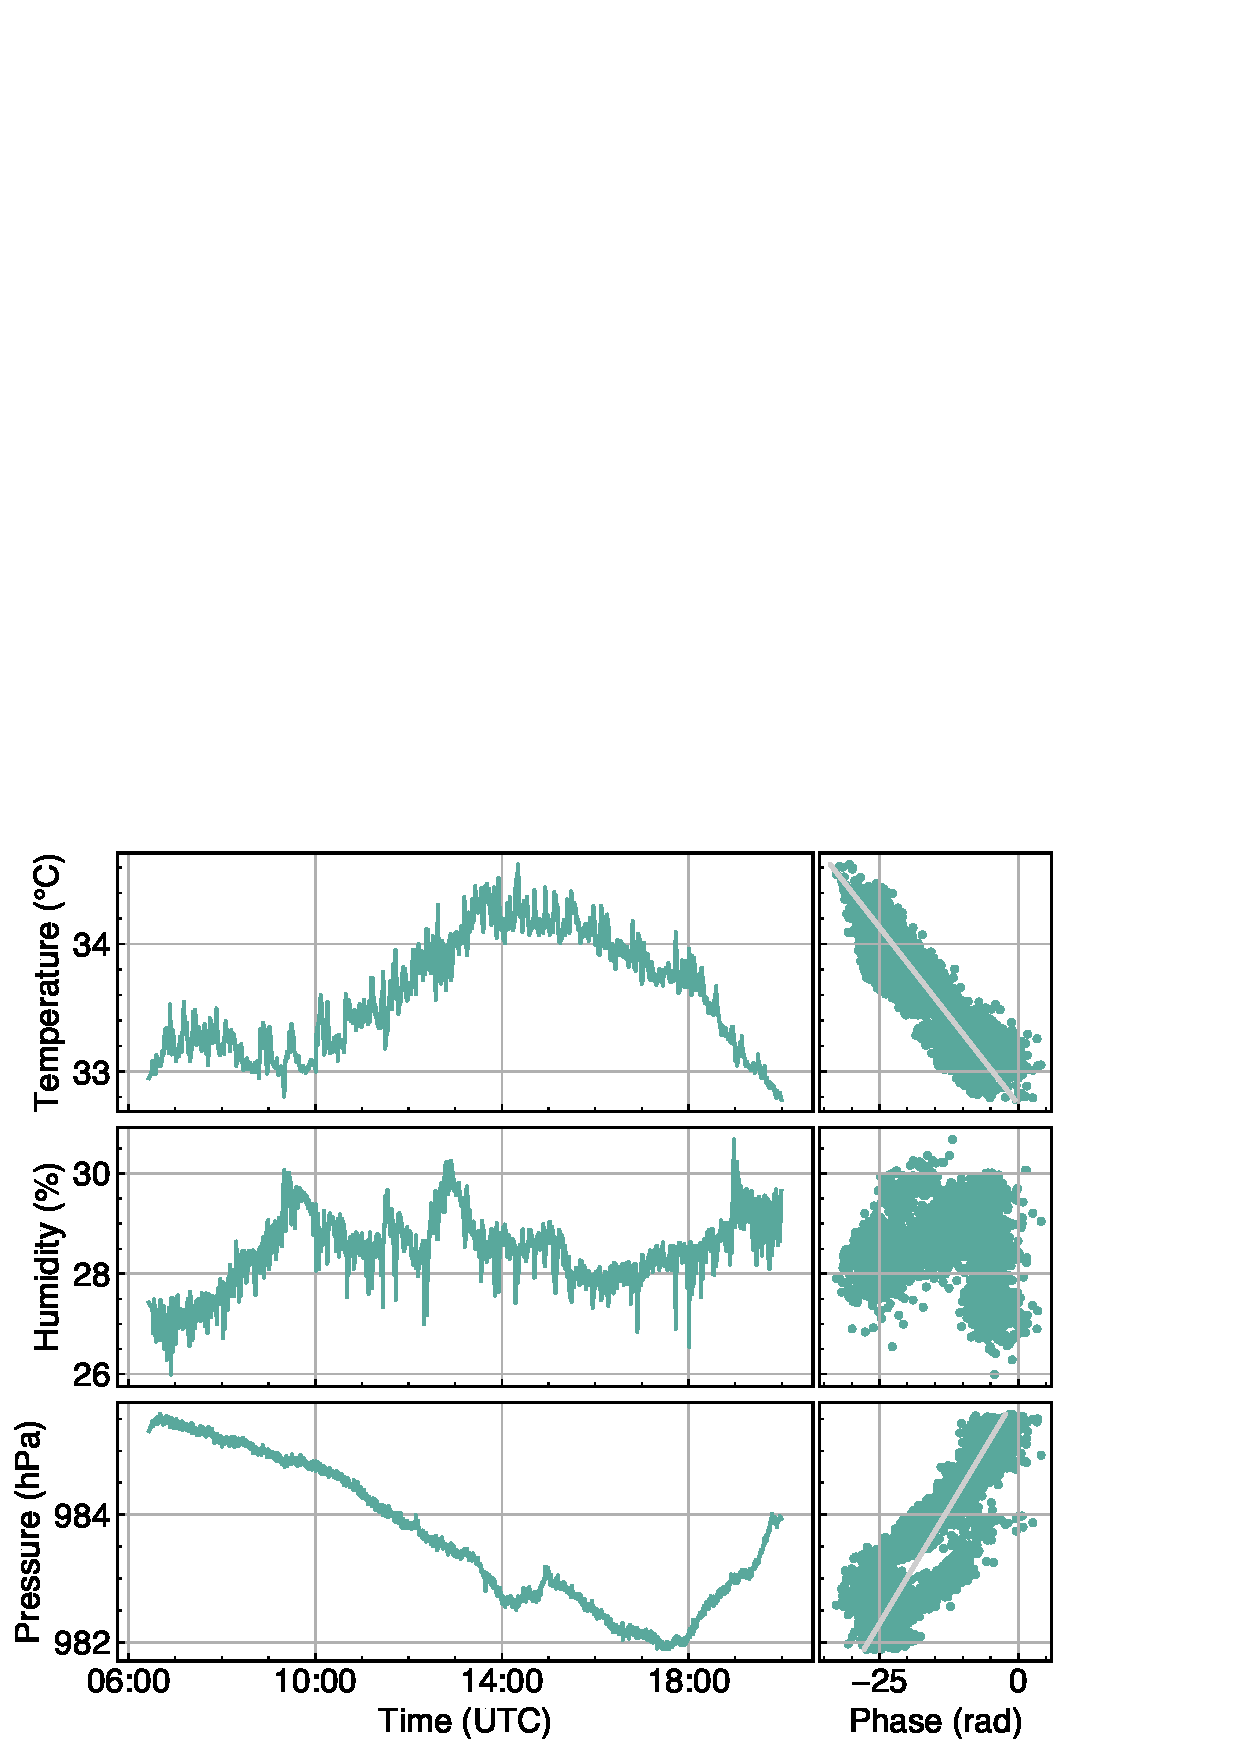
\includegraphics[width=0.8\textwidth]{figures/fig2_new.pdf}
\caption{
Environmental dynamics and their correlations with refractive index at \SI{1762}{\nano\meter}, illustrated using a \SI{14}{\hour} subset of the training dataset.
\textbf{(a--c)} Synchronous \SI{14}{\hour} time-series measurements from the training dataset of atmospheric temperature (\SIrange{33}{34.5}{\celsius}), relative humidity (\SIrange{26}{31}{\percent}), and pressure (\SIrange{982}{986}{\hecto\pascal}) from the training dataset.
\textbf{(d)} Corresponding refractive index variations measured at \SI{1762}{\nano\meter}, expressed as $(n-1.0002)\times 10^{5}$, showing coherent temporal dynamics with environmental parameters.
\textbf{(e--g)} Quantitative correlation analysis between each environmental parameter and the resulting refractive index change. Phase noise exhibits a strong linear dependence on temperature ($R^{2} = 0.828$) and pressure ($R^{2} = 0.751$). The humidity-phase relationship, however, displays a characteristic non-linear pattern, deviating significantly from simple linear modeling.
\textbf{(h)} Self-correlation analysis of refractive index measurements, confirming measurement consistency ($R^{2} = 1.000$) and providing a validation baseline for environmental correlation studies.}
\label{fig:environmental_dynamics}
\end{figure}




\includegraphics[width=0.8\textwidth]{figures/fig2_alt.pdf}


{Alternatively, figure 2 only concludes the raw data, but here it's bringing new difficulty to describe the linear relationship with the ambient parameters.}


\begin{figure}[ht]
\centering
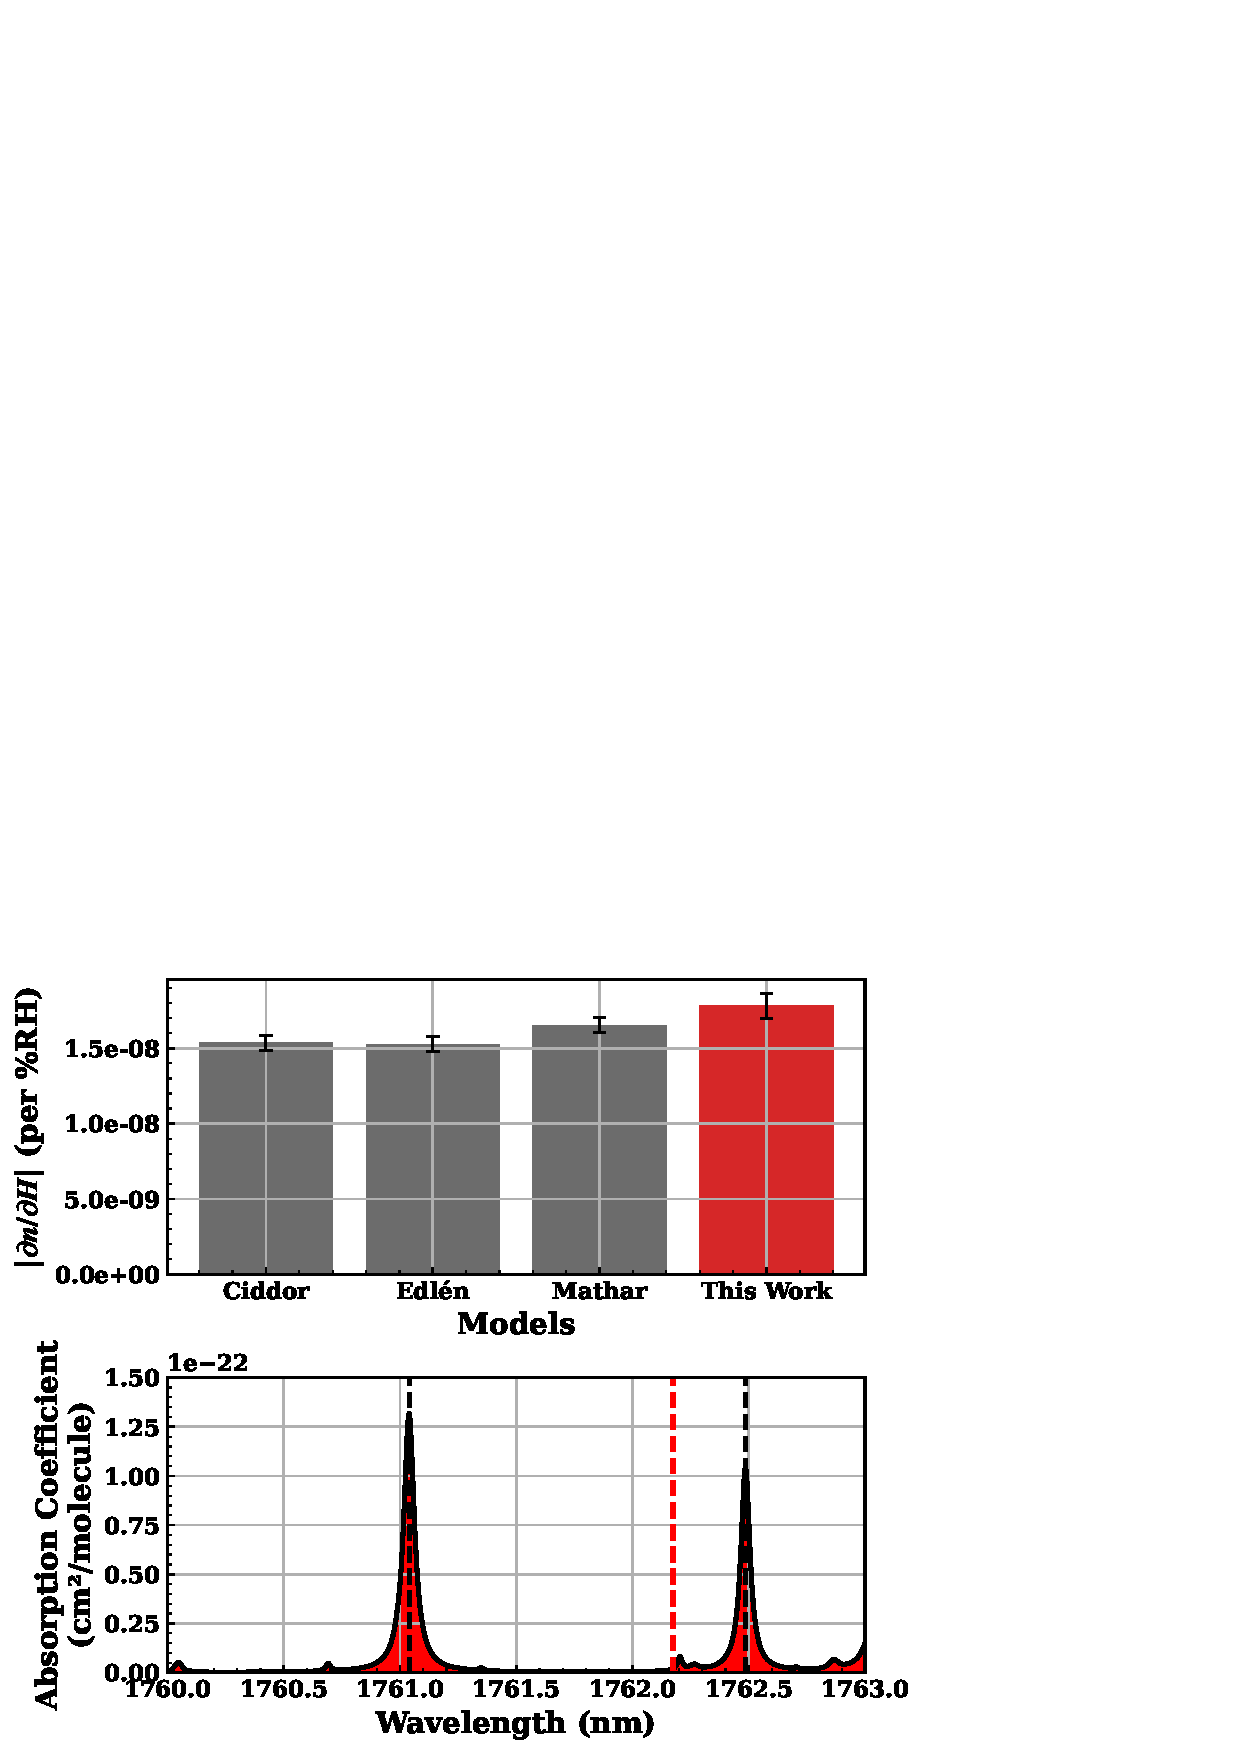
\includegraphics[width=0.8\textwidth]{figures/fig3_humidity_discrepancy.pdf}
\caption{
Systematic discrepancy in humidity sensitivity and its physical origin at \SI{1762}{\nano\meter}.
\textbf{(a)} Comparison of the experimentally derived humidity sensitivity coefficient with predictions from established empirical models. A significant enhancement is identified, while excellent agreement ($<\SI{1}{\percent}$ deviation) is found for temperature and pressure coefficients.
\textbf{(b)} Spectral analysis showing water vapor absorption features in the vicinity of the quantum-critical wavelength. The \SI{1762}{\nano\meter} transition lies between two strong absorption peaks at \SI{1761.0405}{\nano\meter} and \SI{1762.4852}{\nano\meter}, creating ideal conditions for Kramers-Kronig enhanced dispersion. Our first-principles calculation, performed over the full spectral range from \SI{1}{\micro\meter} to \SI{50}{\micro\meter}, explains the observed \SI{15.3}{\percent} increase in humidity sensitivity compared to the Ciddor model, or other standard atmospheric models.
}
\label{fig:humidity_discrepancy}
\end{figure}

\begin{figure}[ht]
\centering
\includegraphics[width=1\textwidth]{figures/combined_figure.png}
\caption{
Multi-scale phase noise characterization and suppression efficacy for quantum applications. 
\textbf{(a)} Long-term (\SI{15}{\day}) phase stability using the full validation dataset: time-domain performance showing environmental noise mitigation, with gray shaded region indicating the fault-tolerant threshold. 
\textbf{(b)} Long-term autocorrelation analysis: correlation time reduced from \SI{5668}{\second} to \SI{302}{\second}. 
\textbf{(c)} Long-term spectral characterization: power spectral density demonstrating substantial low-frequency noise suppression. 
\textbf{(d)} Short-term (\SI{12}{\hour}) phase dynamics from the validation dataset: optimized performance for quantum gate operations, with gray shaded region indicating the fault-tolerant threshold. 
\textbf{(e)} Short-term autocorrelation: dramatic noise whitening with correlation time reduced from \SI{560}{\second} to \SI{1}{\second}. 
\textbf{(f)} Short-term spectral analysis: frequency-domain transformation revealing noise structure modification. 
Key performance metrics: Long-term noise reduction of \SI{80.97}{\percent} ($\sigma_\phi$: \SI{17.938}{\radian} $\rightarrow$ \SI{3.414}{\radian}, 5.3$\times$) optimized for quantum memory applications. Short-term suppression achieves \SI{60.20}{\percent} reduction ($\sigma_\phi$: \SI{6.548}{\radian} $\rightarrow$ \SI{2.606}{\radian}, 2.5$\times$) ideal for quantum gate operations. QEC threshold compliance improved from \SI{1.2}{\percent} to \SI{9.7}{\percent} (long-term) and \SI{3.3}{\percent} to \SI{13.3}{\percent} (short-term). 
}
\label{fig:timeseries_comparison}
\end{figure}

\end{document}
